\section{Pengujian}\label{sec:Pengujian}

Pengujian pada laporan ini dilakukan melalui GUI. Setiap bukti yang
dimasukkan ke laporan berupa tangkapan layar GUI yang memperlihatkan
file testcase yang diunggah, algoritma yang dipilih, heuristic jika
digunakan, panel hasil, board solusi, playback, dan search graph.
Untuk membuktikan fitur penyimpanan solusi, salah satu bukti GUI juga
dapat memperlihatkan tombol \texttt{Save .txt} atau hasil unduhan
berkas solusi.
Testcase utama menggunakan nama file yang sudah disiapkan pada folder
\texttt{test/} sesuai algoritma yang diuji. File
\texttt{testcase\_ucs.txt} dan \texttt{testcase\_astar.txt} memiliki
konfigurasi papan yang sama, tetapi disimpan sebagai file berbeda agar
bukti pengujian per algoritma lebih jelas. Demikian pula
\texttt{testcase\_dfs.txt} dan \texttt{testcase\_bfs.txt}.
\texttt{testcase\_sanity.txt} tetap tersedia sebagai sanity check
sederhana untuk upload dan rendering GUI, tetapi tidak dijadikan bukti
utama karena kasusnya terlalu ringan dibandingkan testcase lain.

\subsection{Rencana Pengujian GUI}\label{sub:Rencana Pengujian GUI}

\begin{table}[H]
    \centering
    \begin{tabular}{|c|L{3cm}|L{3cm}|L{5cm}|}
        \hline
        \textbf{No} & \textbf{File} & \textbf{Algoritma} & \textbf{Tujuan} \\
        \hline
        1 & \texttt{testcase\_ucs.txt} & UCS & Menguji pencarian berbasis cost pada papan dengan checkpoint dan lava. \\
        \hline
        2 & \texttt{testcase\_gbfs.txt} & GBFS H1, H2, H3 & Menguji seluruh heuristic GBFS pada papan lebih besar dengan tiga checkpoint. \\
        \hline
        3 & \texttt{testcase\_astar.txt} & A* H1, H2, H3 & Menguji seluruh heuristic A* pada papan berbobot dengan checkpoint. \\
        \hline
        4 & \texttt{testcase\_dfs.txt} & DFS & Menguji algoritma bonus DFS pada papan non-persegi. \\
        \hline
        5 & \texttt{testcase\_bfs.txt} & BFS & Menguji algoritma bonus BFS pada papan non-persegi. \\
        \hline
    \end{tabular}
    \caption{Rencana pengujian algoritma melalui GUI}
\end{table}

\subsection{Format Bukti Pengujian}\label{sub:Format Bukti Pengujian}

Setiap bukti GUI dilengkapi dengan informasi berikut.
\begin{itemize}[label=\textbullet]
    \item file testcase yang diunggah;
    \item algoritma dan heuristic yang dipilih;
    \item status solusi ditemukan;
    \item moves, total cost, jumlah iterasi, dan waktu eksekusi;
    \item tampilan board pada salah satu step playback;
    \item tampilan search graph;
    \item tombol atau hasil penyimpanan solusi \texttt{.txt} untuk
        minimal satu pengujian.
\end{itemize}

\pagebreak

\subsection{Kasus Uji 1: UCS pada \texttt{testcase\_ucs.txt}}\label{sub:Kasus Uji UCS}

\begin{itemize}
    \item File testcase: \texttt{test/testcase\_ucs.txt}.
    \item Algoritma: \texttt{UCS}.
    \item Heuristic: tidak digunakan.
    \item Kompleksitas kasus: papan $7 \times 7$, terdapat checkpoint
        \texttt{0} dan \texttt{1}, lava, dinding, serta cost tile yang
        bervariasi.
    \item Ekspektasi: GUI menampilkan solusi dengan total cost minimum
        berdasarkan UCS.
\end{itemize}

\begin{figure}[H]
    \centering
    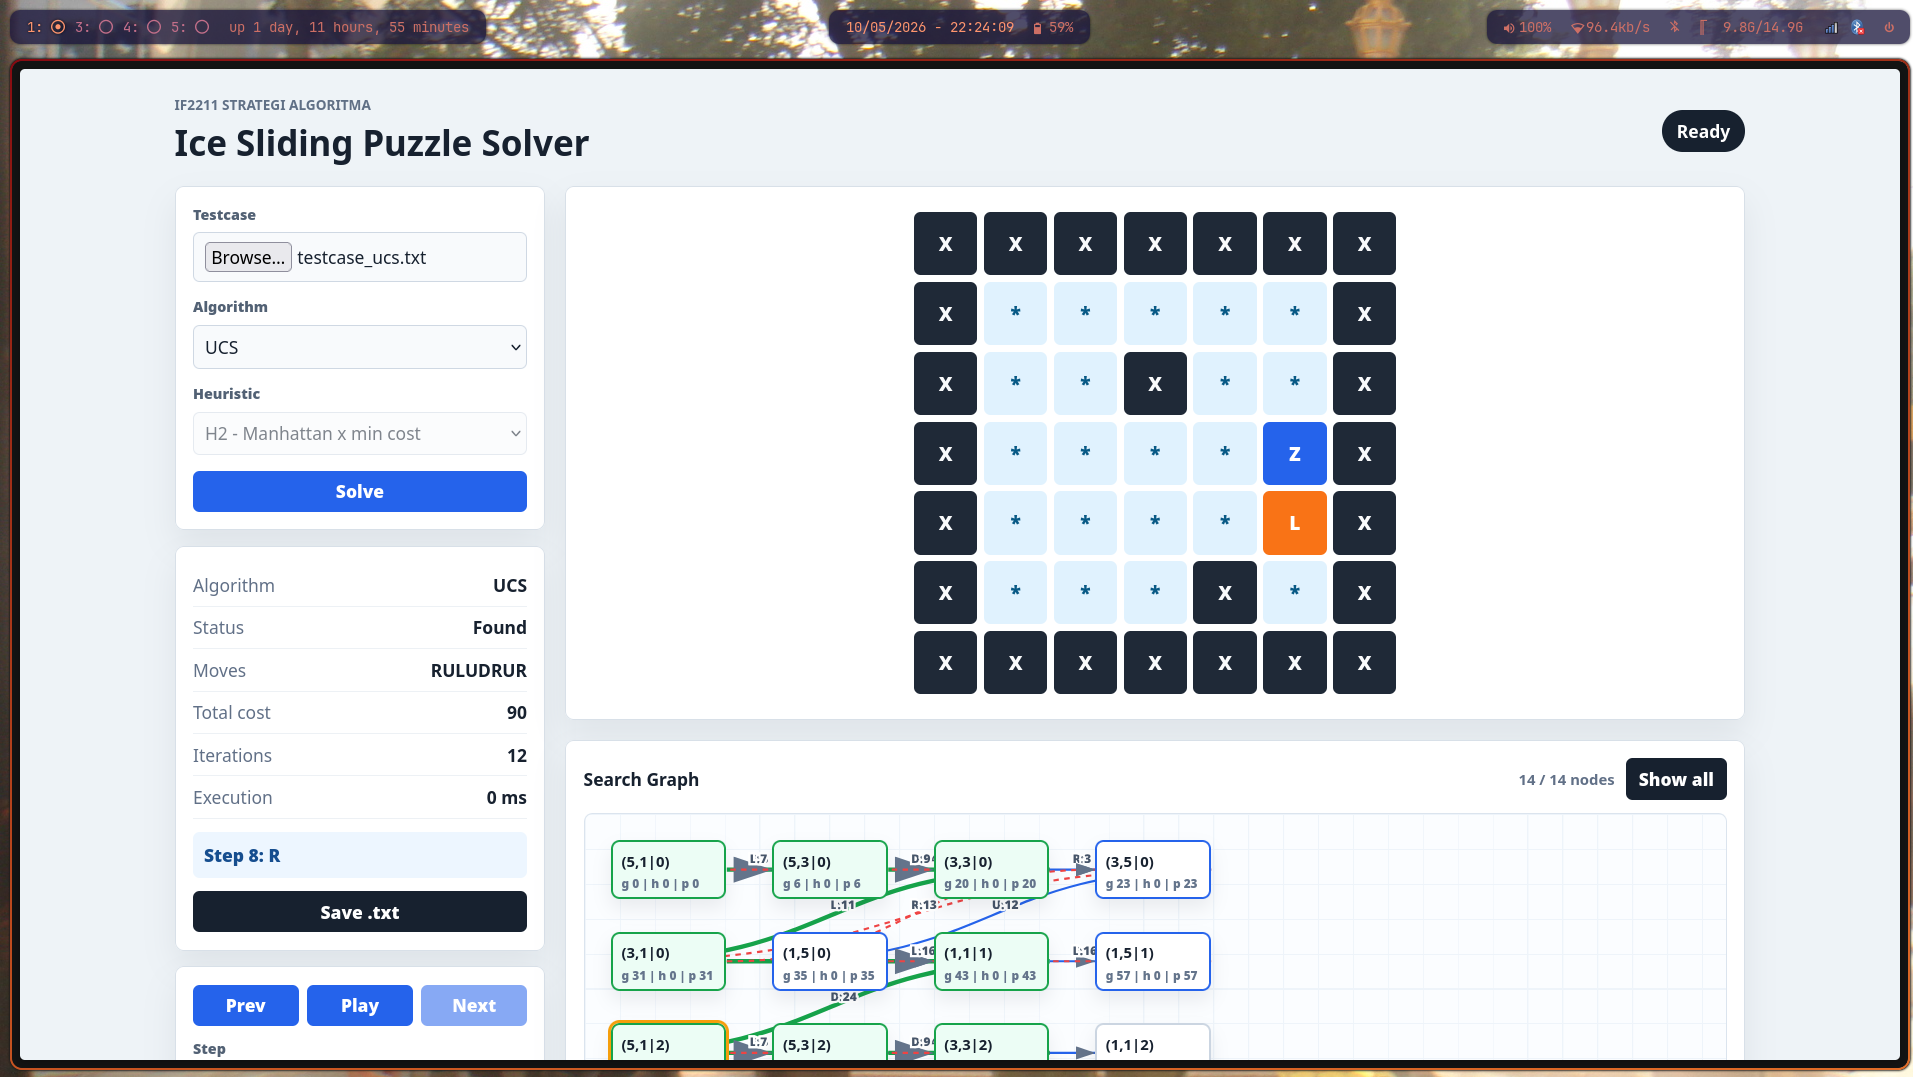
\includegraphics[width=0.85\textwidth]{figures/testcase_ucs.png}
    \caption{Bukti GUI UCS pada \texttt{testcase\_ucs.txt}}
\end{figure}

\subsection{Kasus Uji 2: GBFS H1, H2, dan H3 pada \texttt{testcase\_gbfs.txt}}\label{sub:Kasus Uji GBFS}

\begin{itemize}
    \item File testcase: \texttt{test/testcase\_gbfs.txt}.
    \item Algoritma: \texttt{GBFS}.
    \item Heuristic yang diuji: \texttt{H1}, \texttt{H2}, dan
        \texttt{H3}.
    \item Kompleksitas kasus: papan $8 \times 9$ dengan checkpoint
        \texttt{0}, \texttt{1}, dan \texttt{2}; jalur dibatasi oleh
        banyak dinding sehingga urutan checkpoint harus benar.
    \item Ekspektasi: setiap heuristic dapat menghasilkan respons
        valid dan GUI menampilkan solusi beserta search graph.
\end{itemize}

\begin{figure}[H]
    \centering
    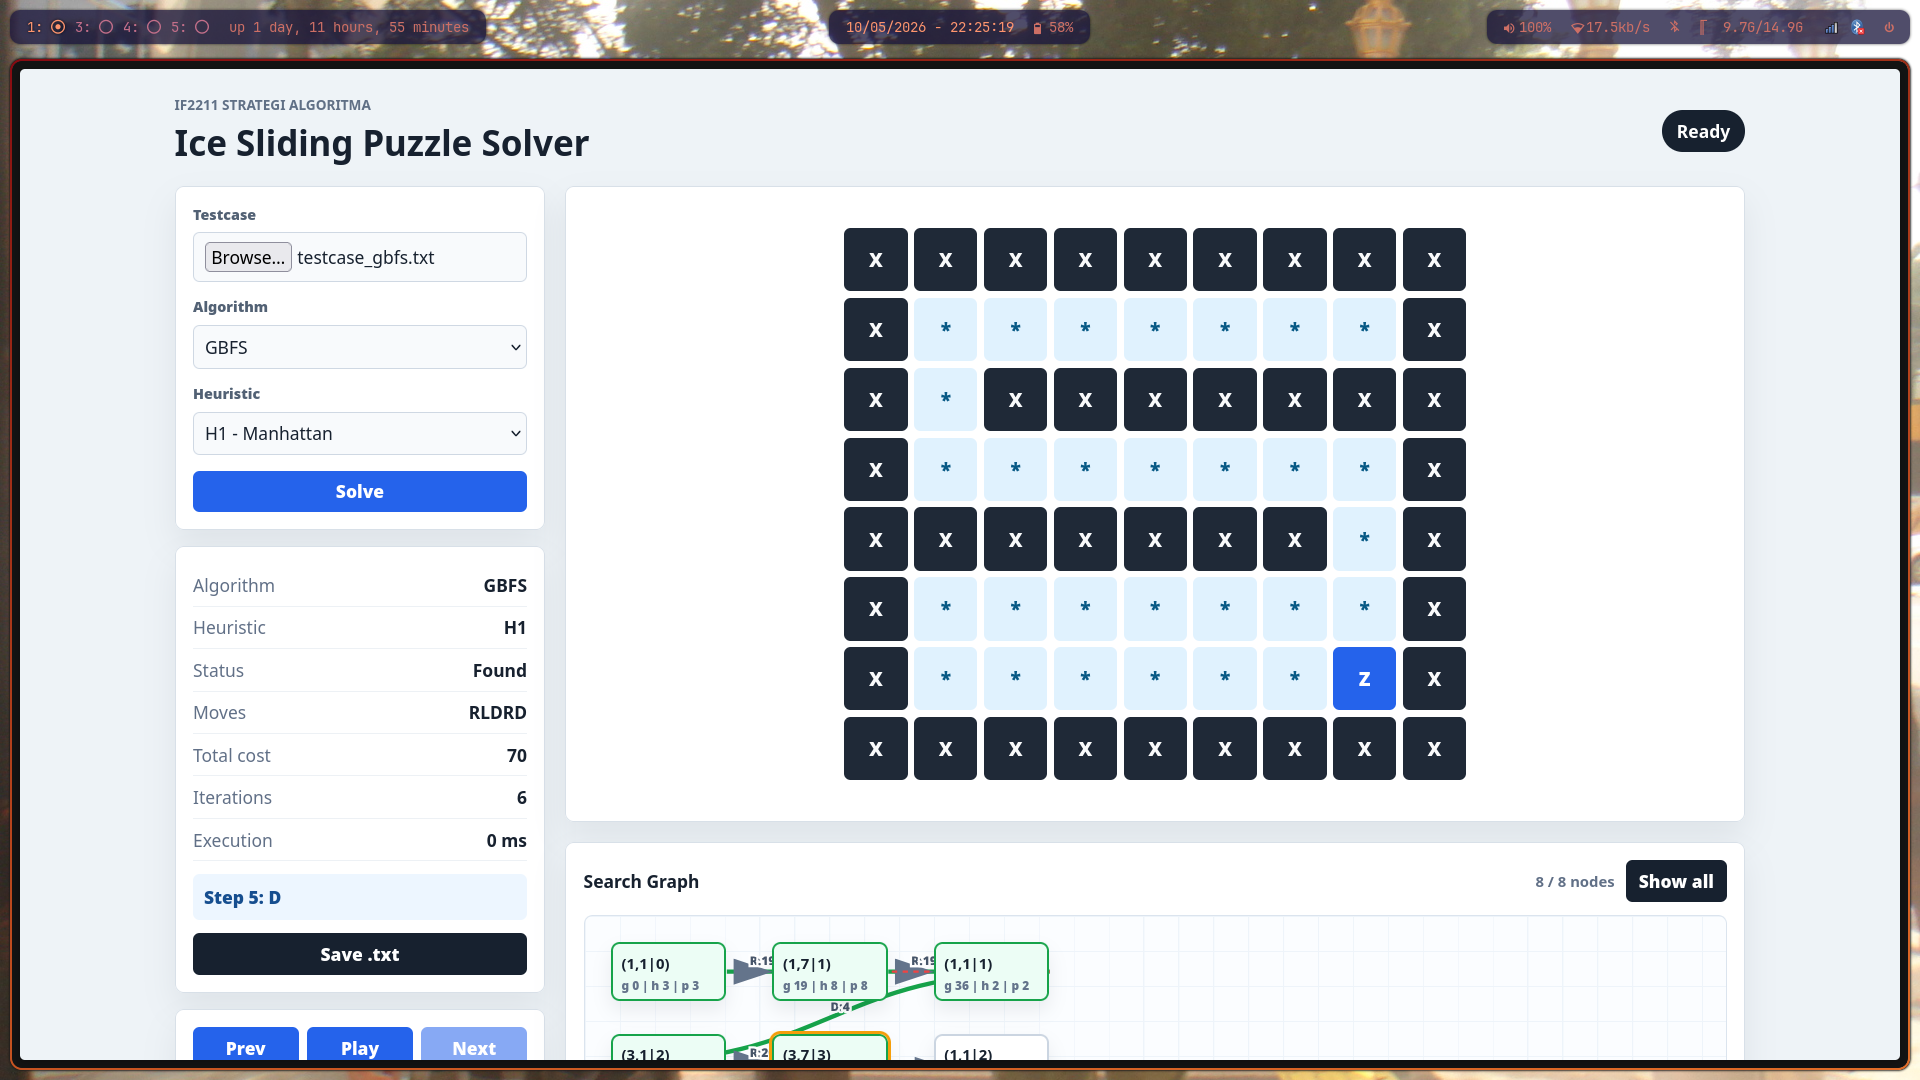
\includegraphics[width=0.85\textwidth]{figures/testcase_gbfs_h1.png}
    \caption{Bukti GUI GBFS H1 pada \texttt{testcase\_gbfs.txt}}
\end{figure}

\begin{figure}[H]
    \centering
    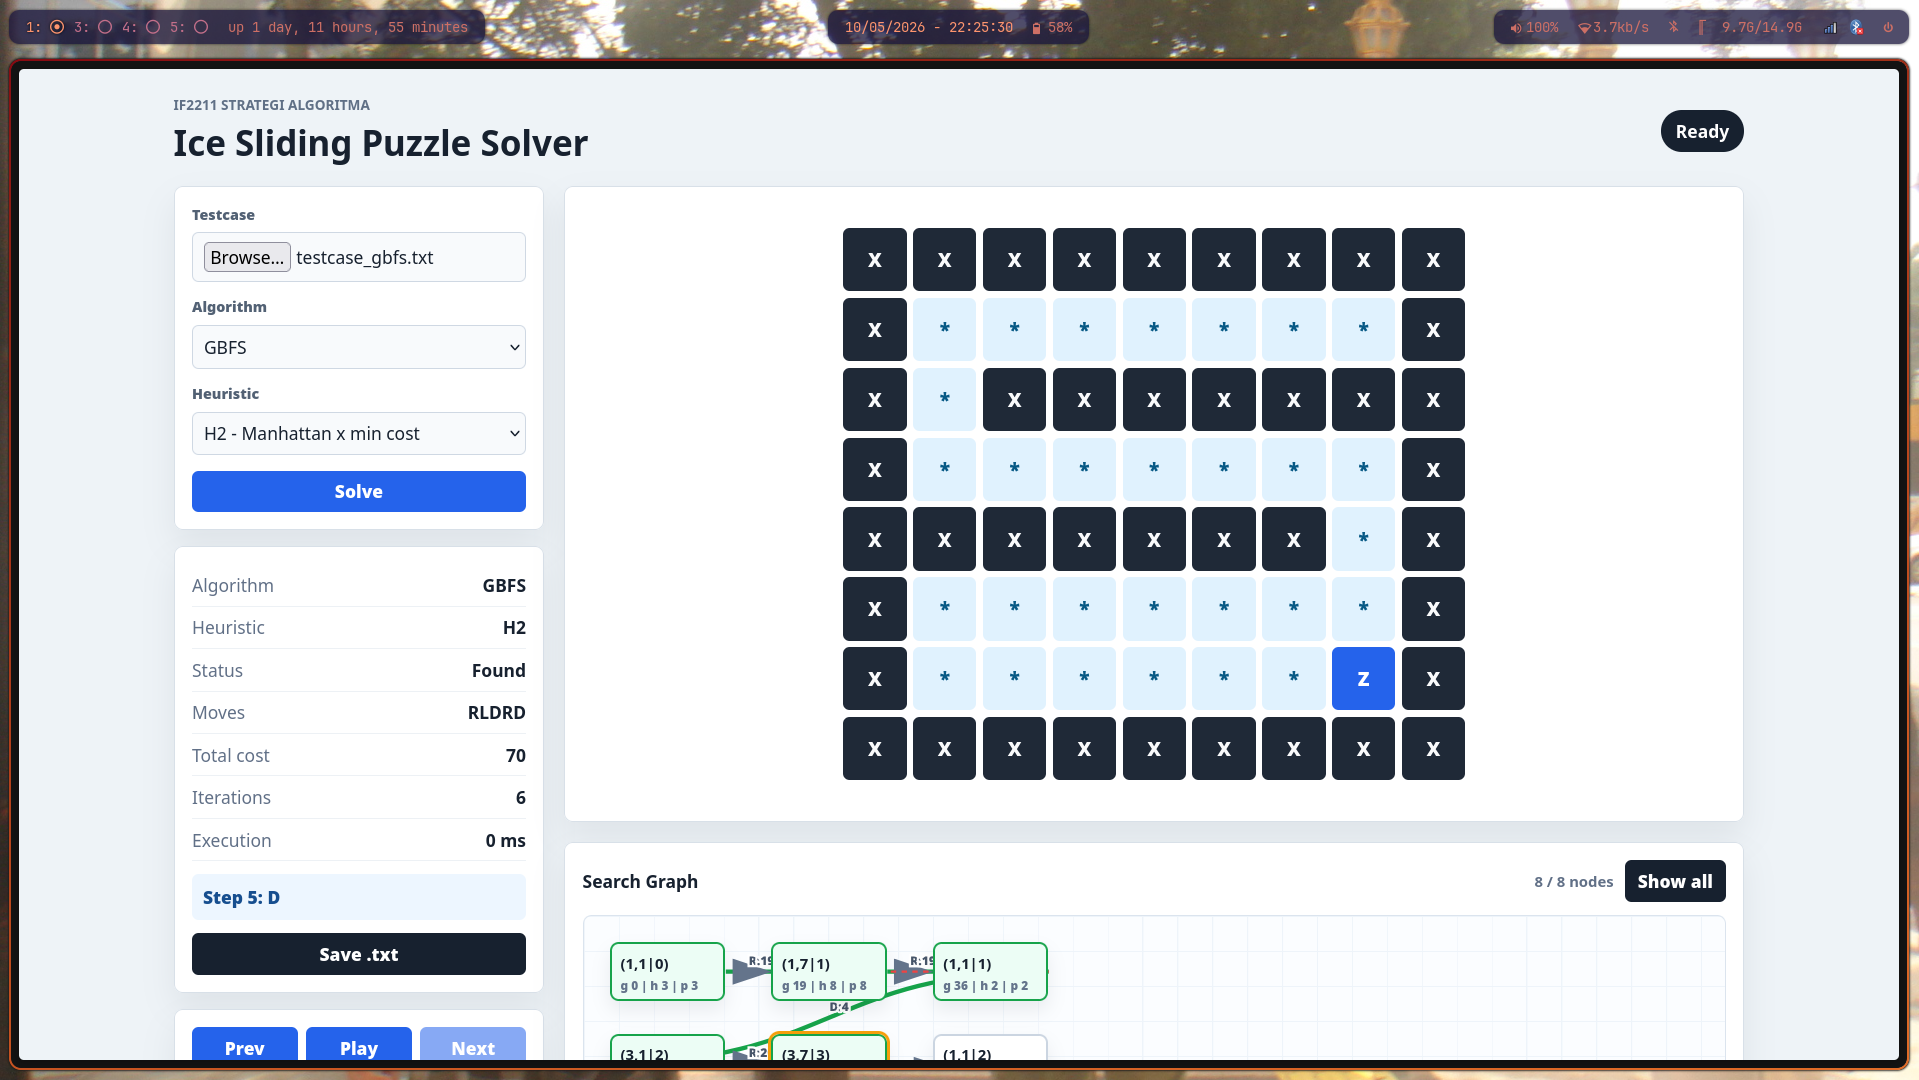
\includegraphics[width=0.85\textwidth]{figures/testcase_gbfs_h2.png}
    \caption{Bukti GUI GBFS H2 pada \texttt{testcase\_gbfs.txt}}
\end{figure}

\begin{figure}[H]
    \centering
    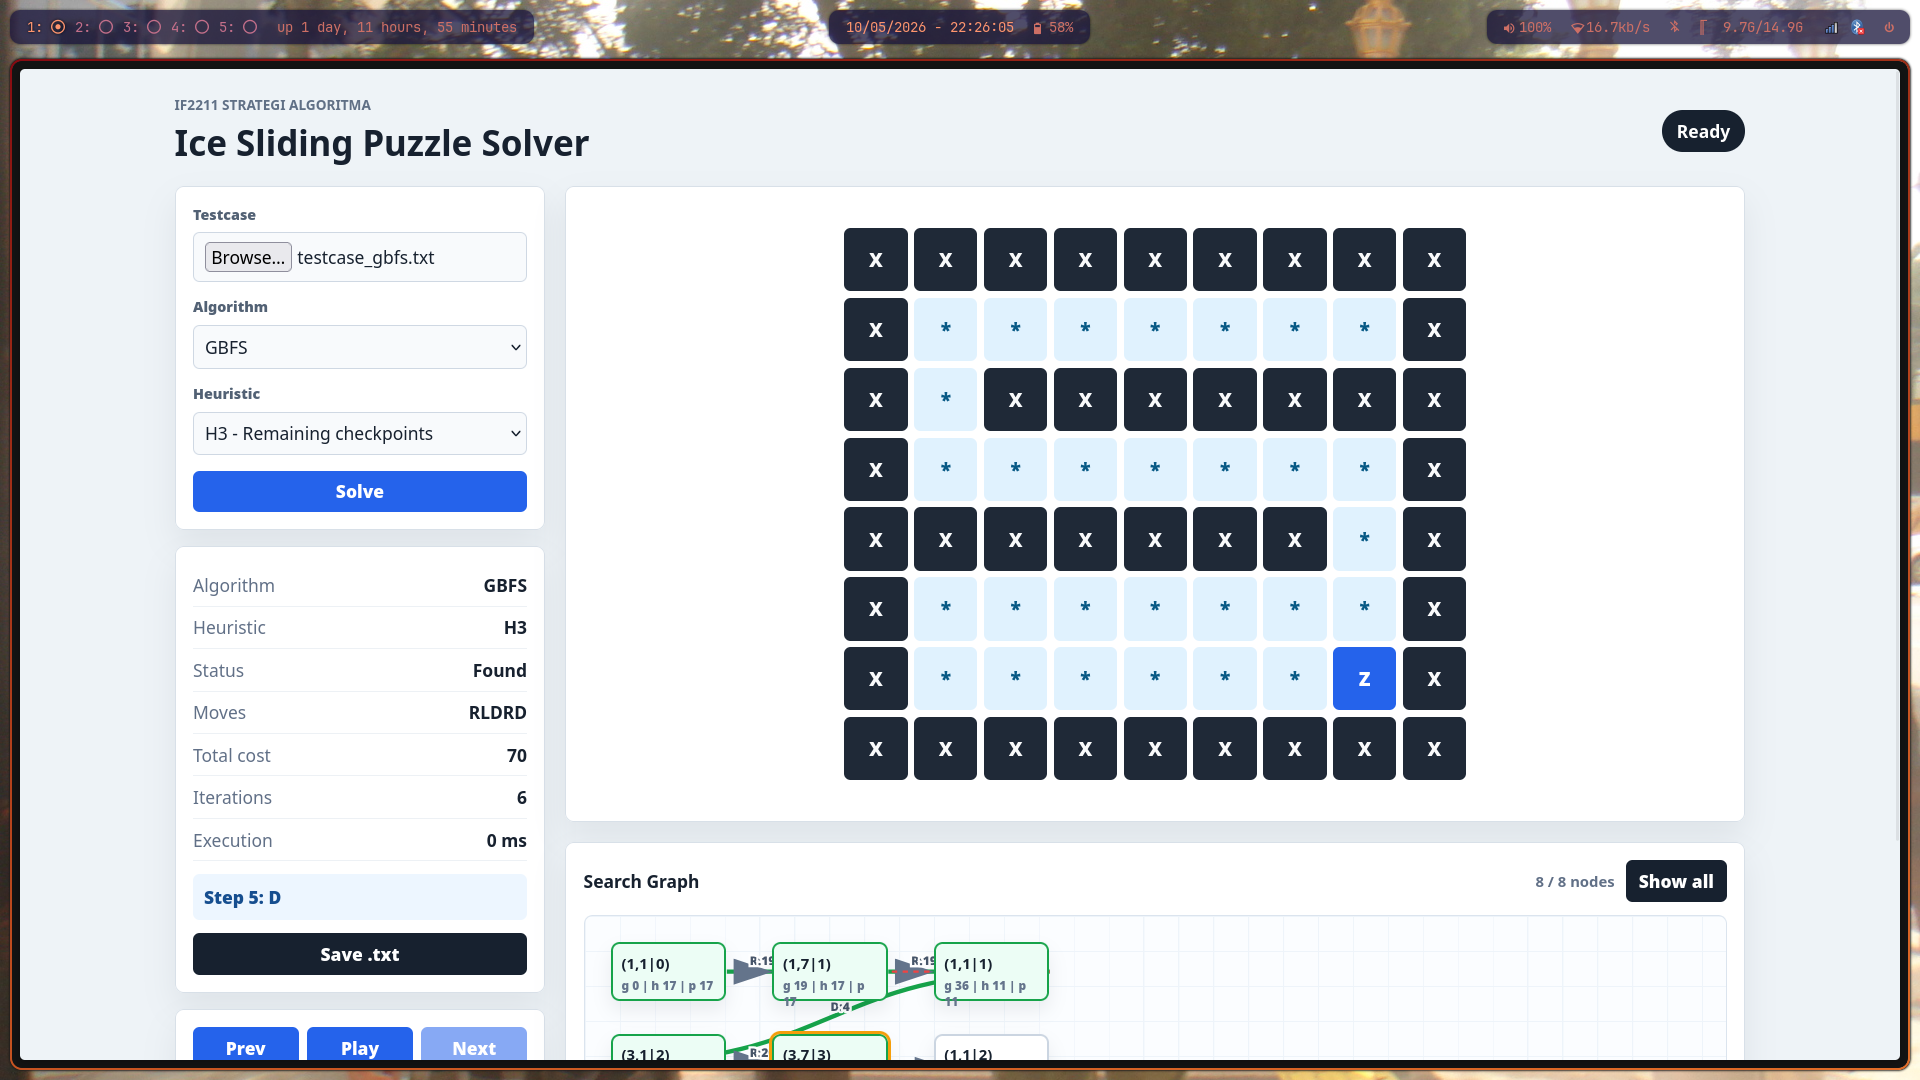
\includegraphics[width=0.85\textwidth]{figures/testcase_gbfs_h3.png}
    \caption{Bukti GUI GBFS H3 pada \texttt{testcase\_gbfs.txt}}
\end{figure}

\subsection{Kasus Uji 3: A* H1, H2, dan H3 pada \texttt{testcase\_astar.txt}}\label{sub:Kasus Uji AStar}

\begin{itemize}
    \item File testcase: \texttt{test/testcase\_astar.txt}.
    \item Algoritma: \texttt{A*}.
    \item Heuristic yang diuji: \texttt{H1}, \texttt{H2}, dan
        \texttt{H3}.
    \item Kompleksitas kasus: papan berbobot dengan checkpoint dan
        lava, sehingga A* harus memperhitungkan $g(n)$ dan $h(n)$.
    \item Ekspektasi: setiap heuristic berjalan lancar dan menghasilkan
        solusi yang dapat divisualisasikan melalui playback GUI.
\end{itemize}

\begin{figure}[H]
    \centering
    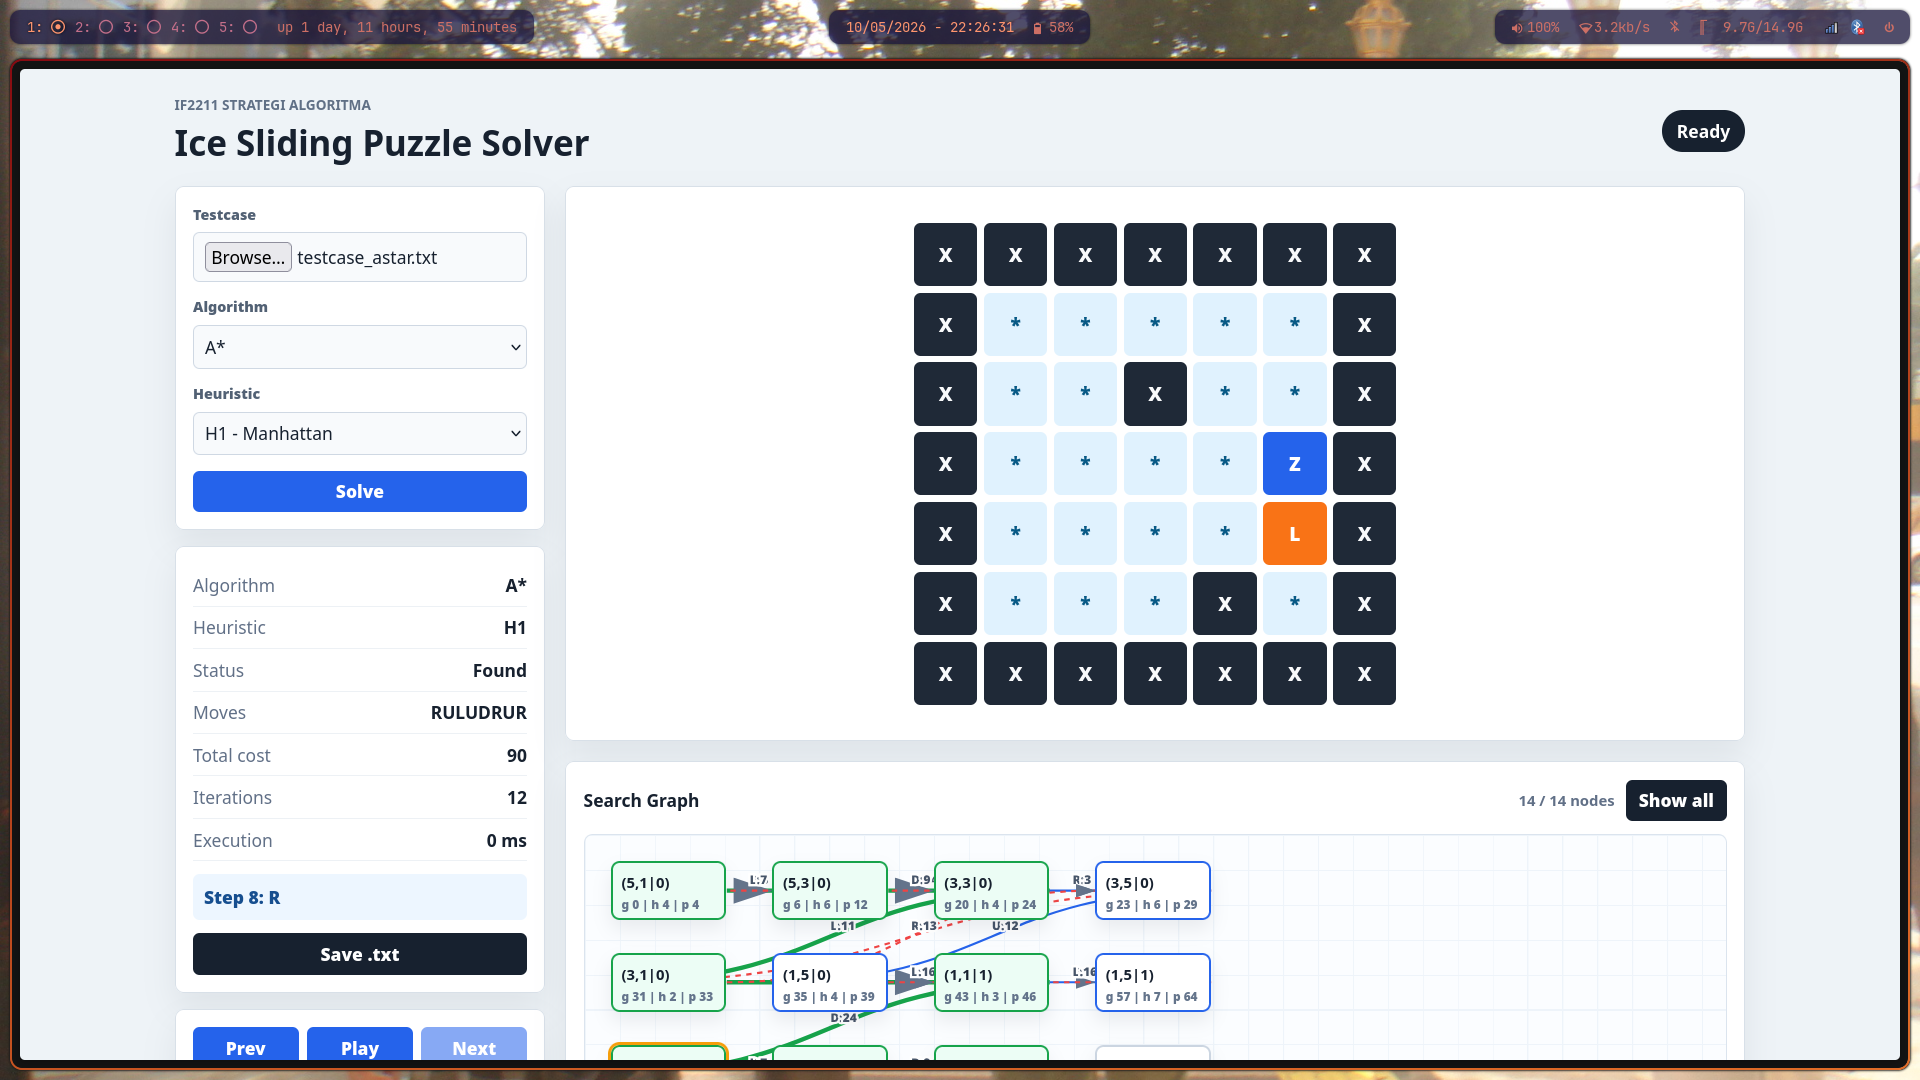
\includegraphics[width=0.85\textwidth]{figures/testcase_astar_h1.png}
    \caption{Bukti GUI A* H1 pada \texttt{testcase\_astar.txt}}
\end{figure}

\begin{figure}[H]
    \centering
    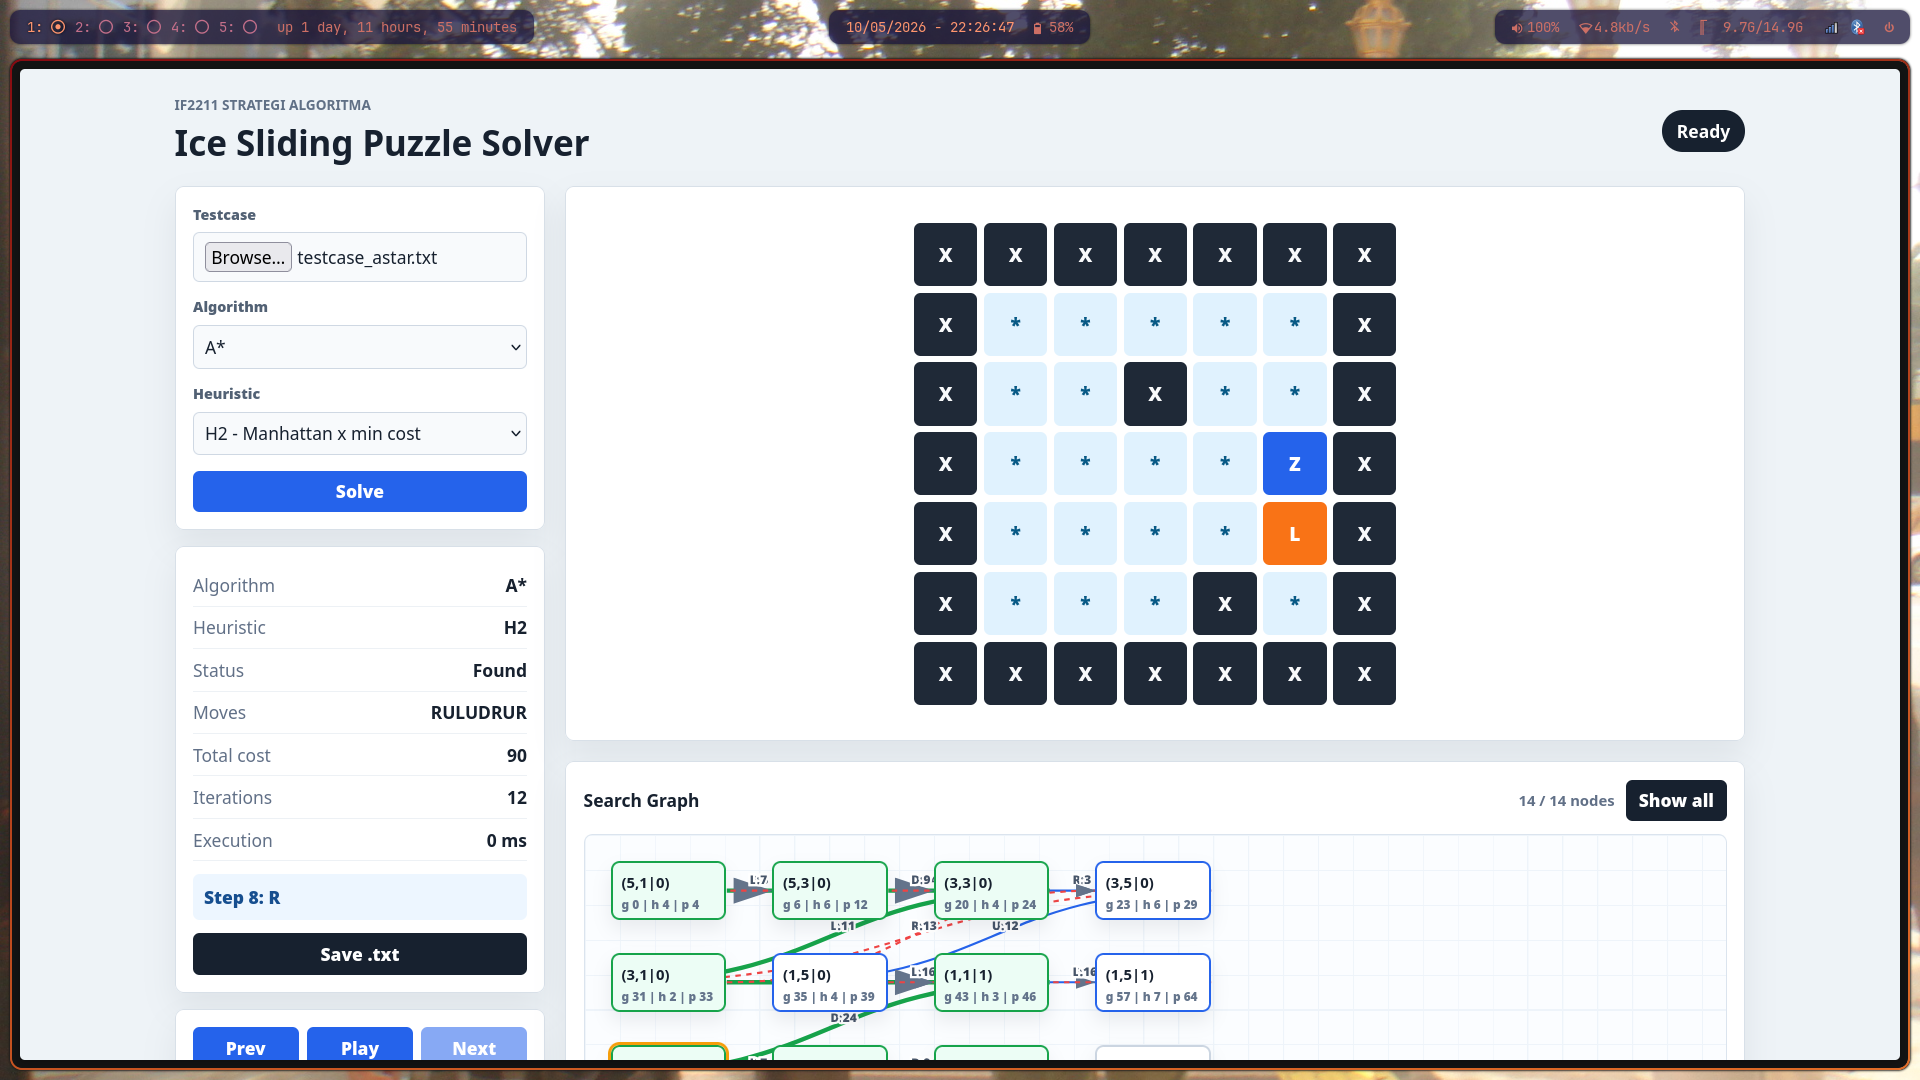
\includegraphics[width=0.85\textwidth]{figures/testcase_astar_h2.png}
    \caption{Bukti GUI A* H2 pada \texttt{testcase\_astar.txt}}
\end{figure}

\begin{figure}[H]
    \centering
    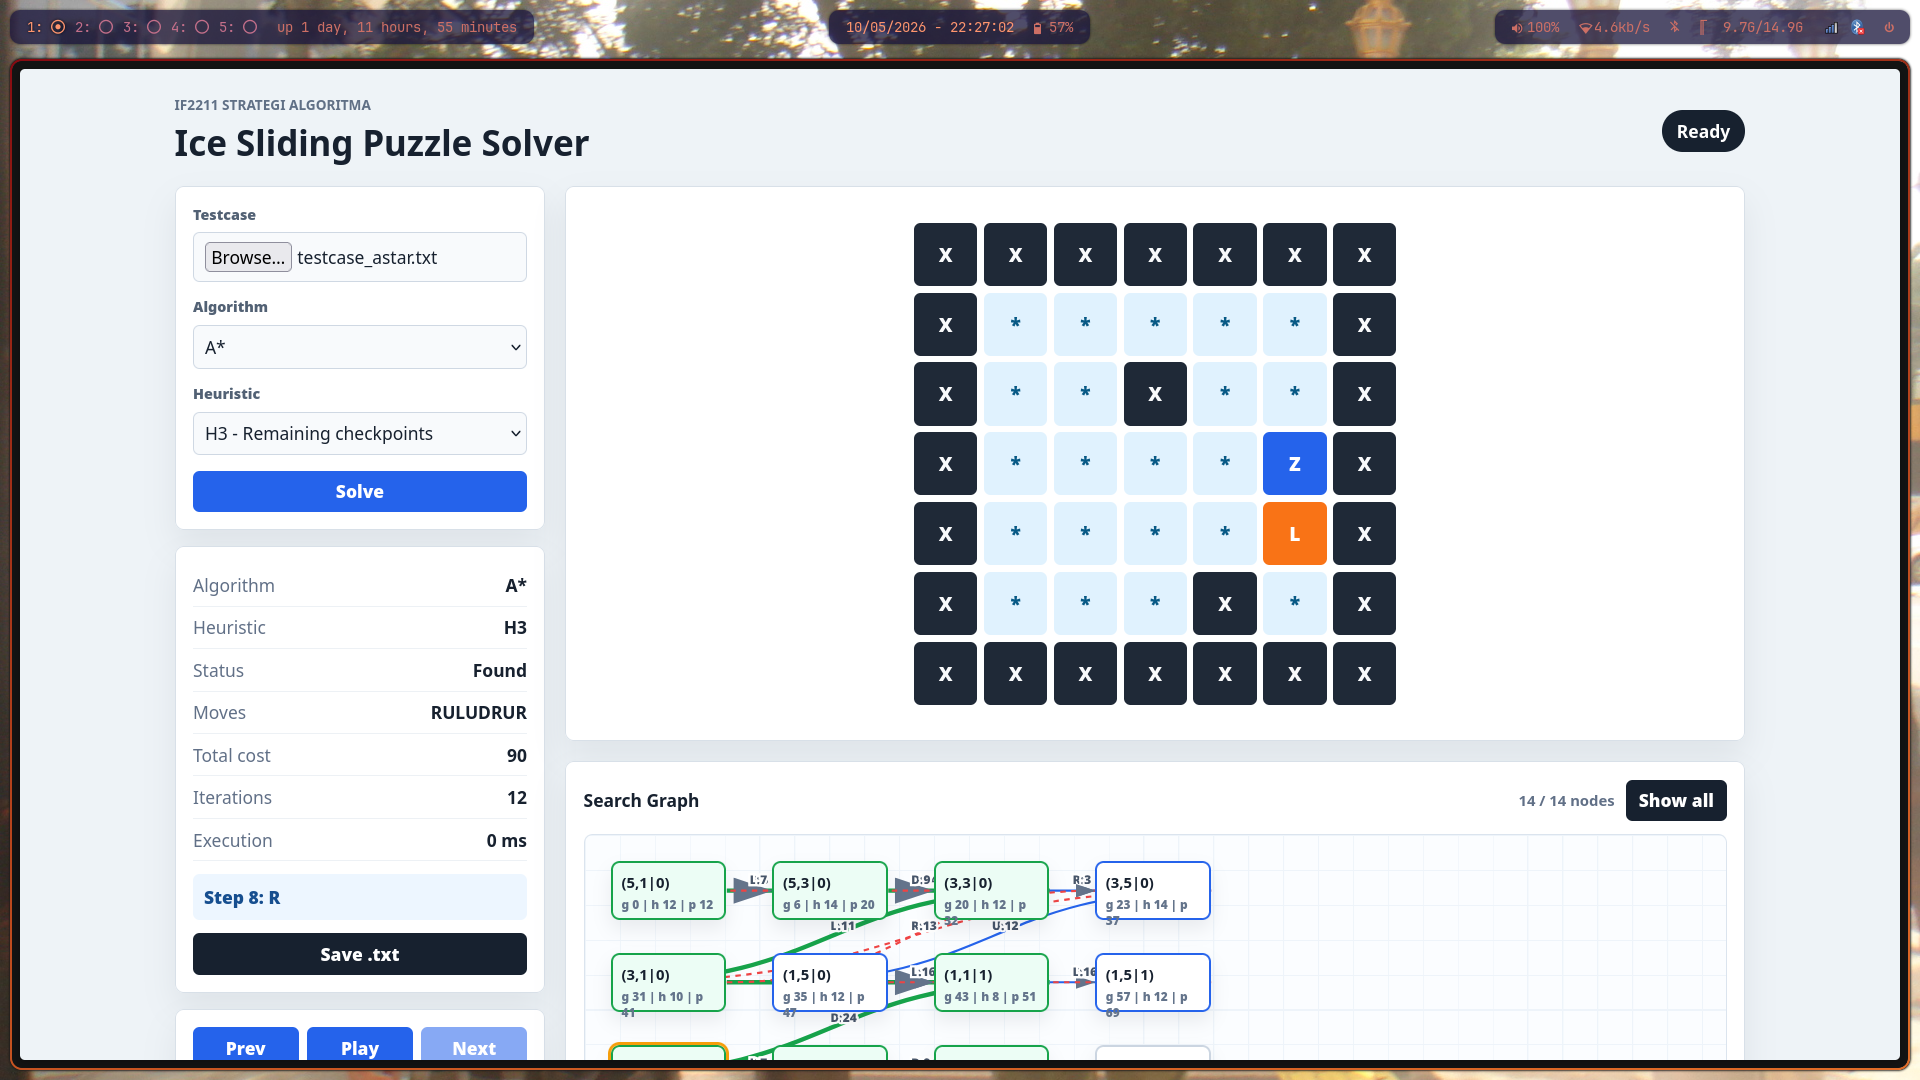
\includegraphics[width=0.85\textwidth]{figures/testcase_astar_h3.png}
    \caption{Bukti GUI A* H3 pada \texttt{testcase\_astar.txt}}
\end{figure}

\subsection{Kasus Uji 4: DFS pada \texttt{testcase\_dfs.txt}}\label{sub:Kasus Uji DFS}

\begin{itemize}
    \item File testcase: \texttt{test/testcase\_dfs.txt}.
    \item Algoritma: \texttt{DFS}.
    \item Heuristic: tidak digunakan.
    \item Kompleksitas kasus: papan non-persegi $5 \times 7$ dengan
        checkpoint \texttt{0}; digunakan untuk memastikan program tidak
        hanya berjalan pada papan persegi.
    \item Ekspektasi: GUI menampilkan solusi valid. Solusi DFS tidak
        harus optimal terhadap total cost maupun jumlah slide.
\end{itemize}

\begin{figure}[H]
    \centering
    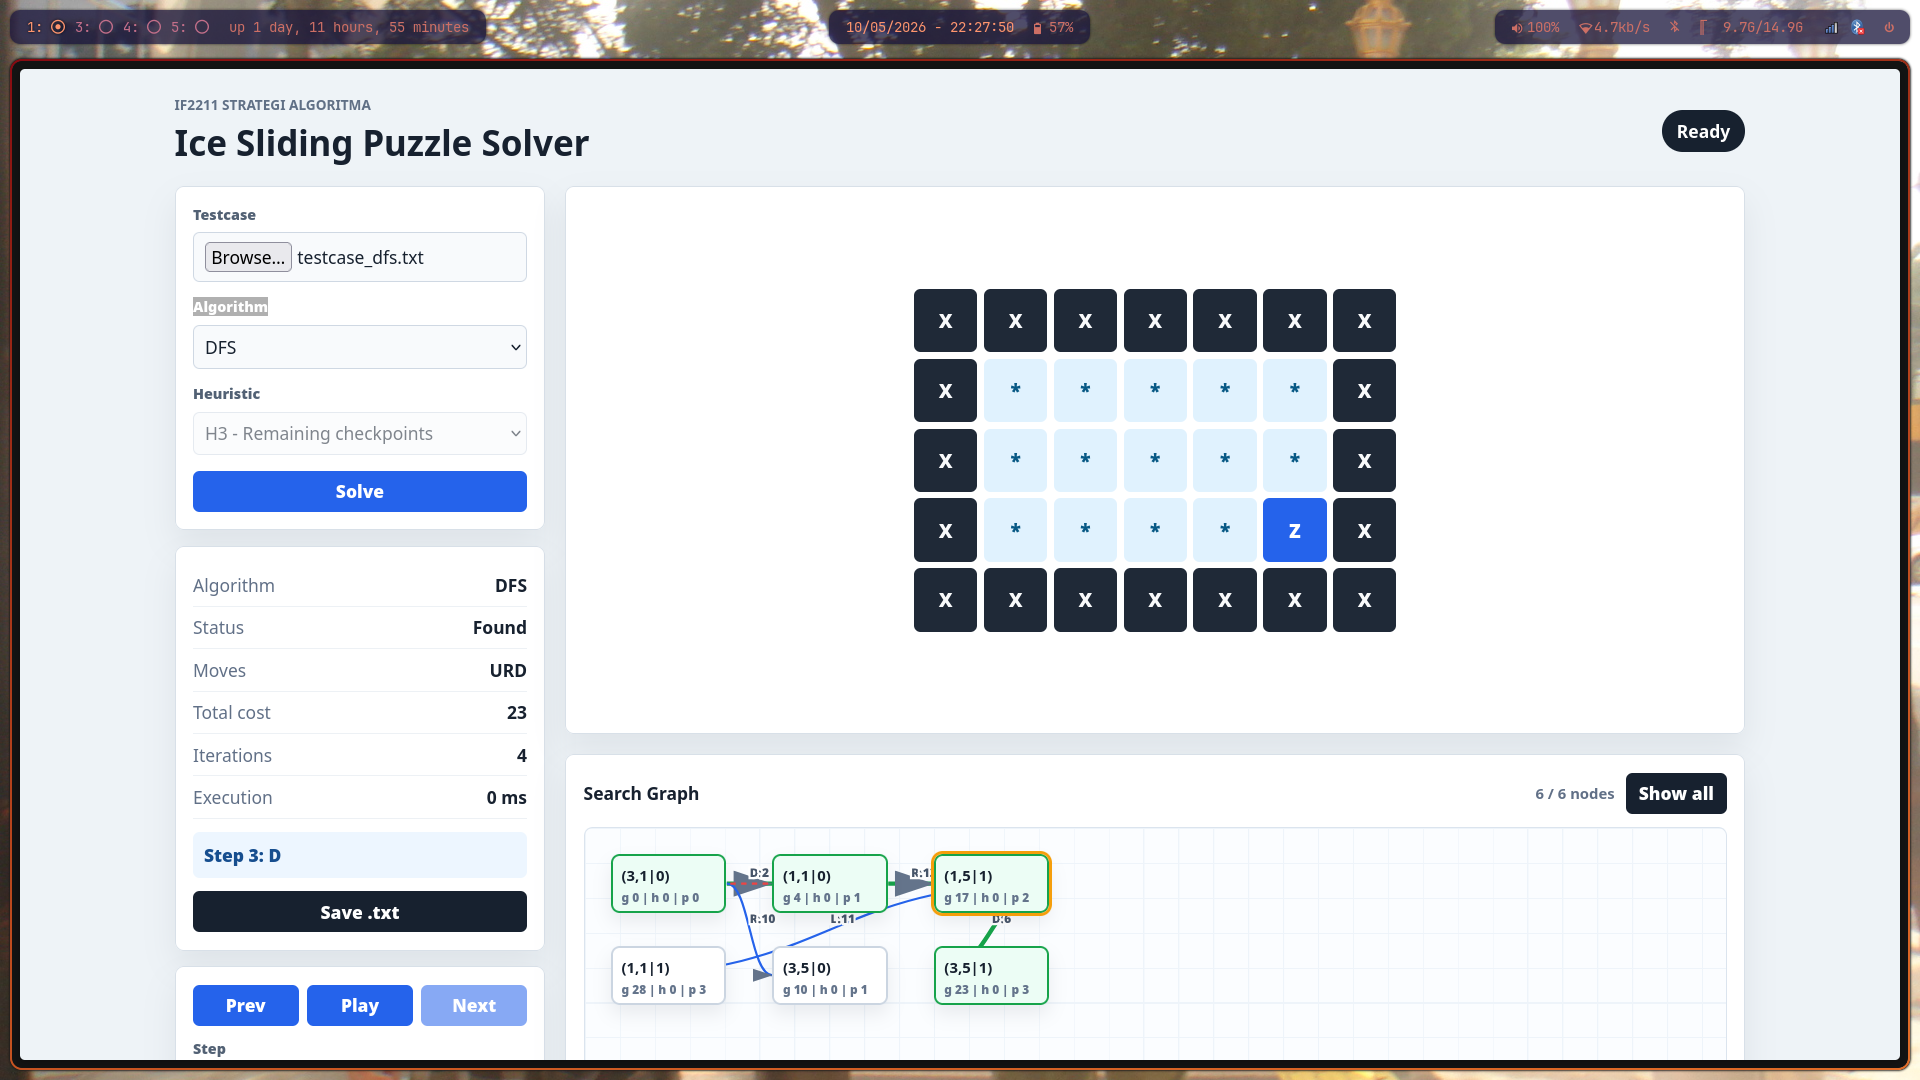
\includegraphics[width=0.85\textwidth]{figures/testcase_dfs.png}
    \caption{Bukti GUI DFS pada \texttt{testcase\_dfs.txt}}
\end{figure}

\subsection{Kasus Uji 5: BFS pada \texttt{testcase\_bfs.txt}}\label{sub:Kasus Uji BFS}

\begin{itemize}
    \item File testcase: \texttt{test/testcase\_bfs.txt}.
    \item Algoritma: \texttt{BFS}.
    \item Heuristic: tidak digunakan.
    \item Kompleksitas kasus: papan non-persegi dengan checkpoint,
        sehingga BFS diuji pada ruang status yang tidak hanya berisi
        start dan goal.
    \item Ekspektasi: GUI menampilkan solusi valid dengan jumlah slide
        minimum pada model pencarian BFS.
\end{itemize}

\begin{figure}[H]
    \centering
    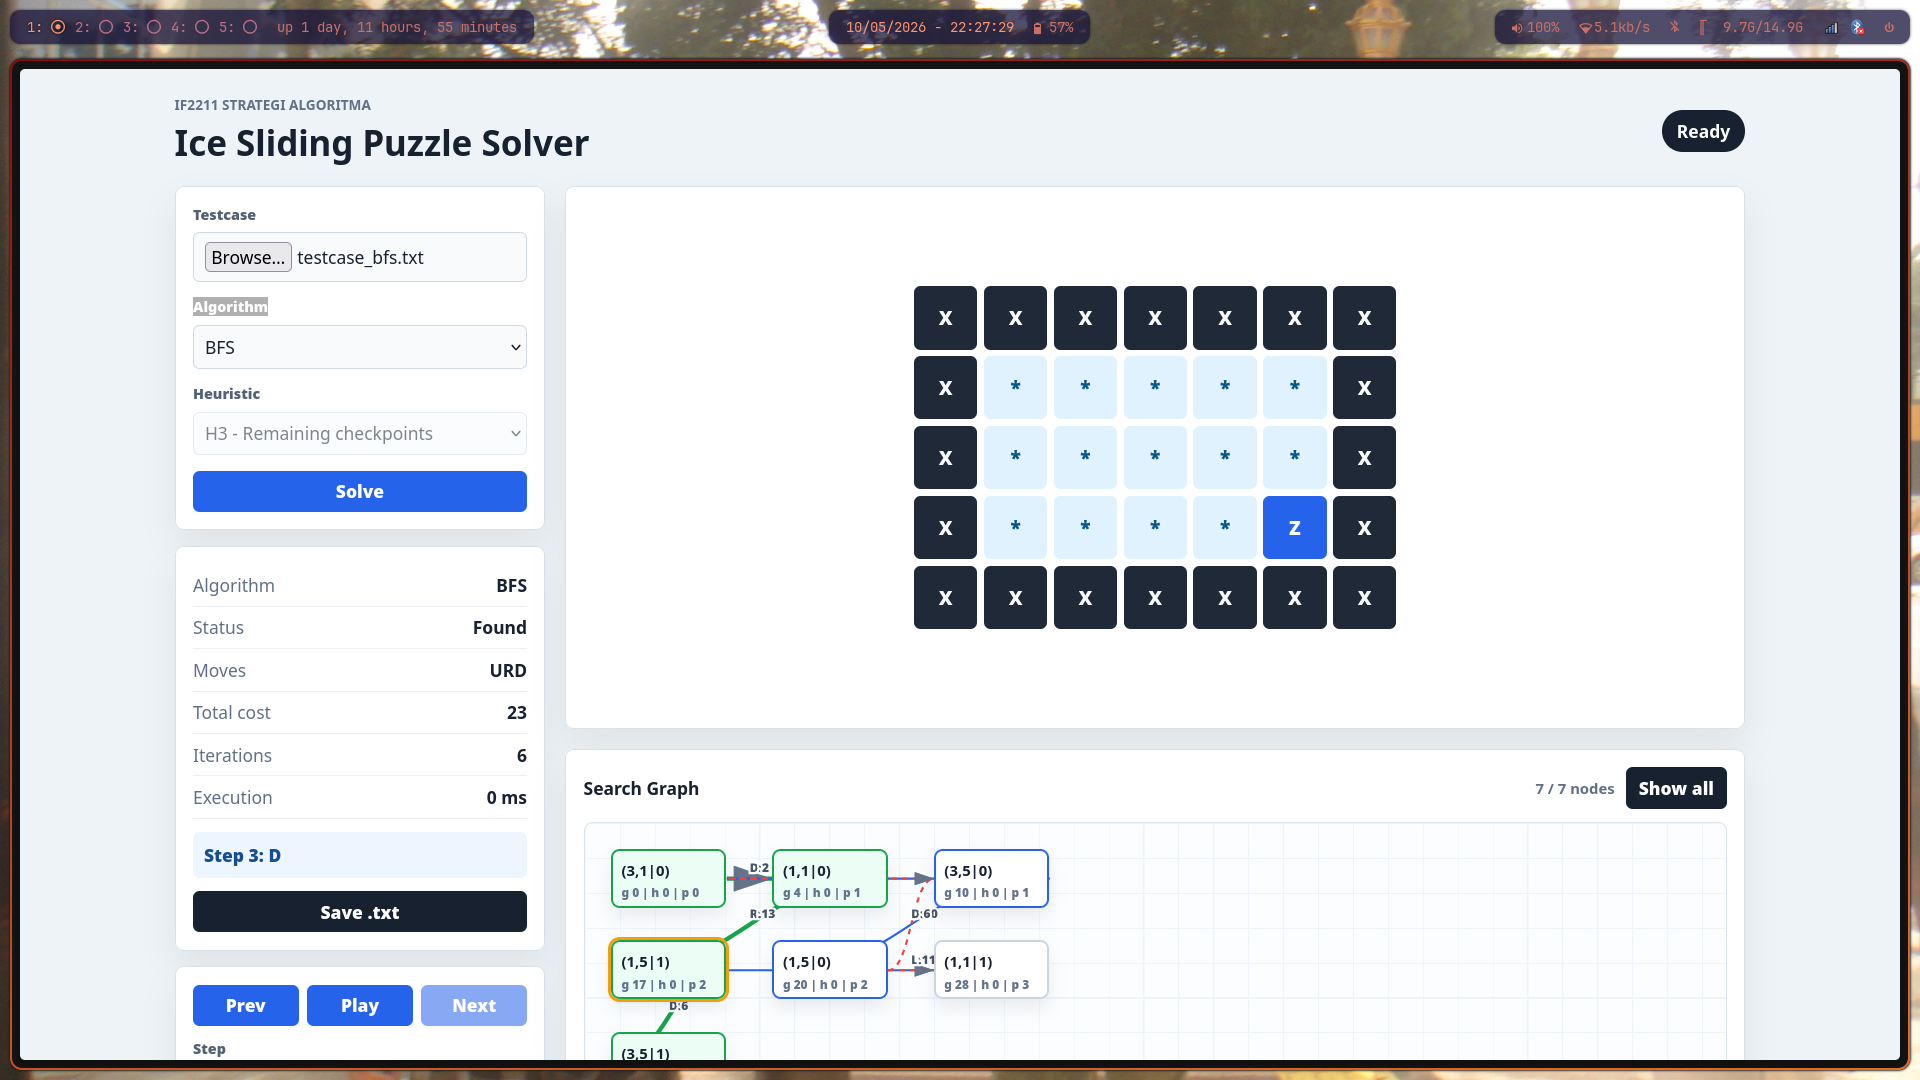
\includegraphics[width=0.85\textwidth]{figures/testcase_bfs.png}
    \caption{Bukti GUI BFS pada \texttt{testcase\_bfs.txt}}
\end{figure}

\subsection{Pengujian Edge Case dan Error Handling}\label{sub:Pengujian Edge Case}

Selain testcase yang menghasilkan solusi, dilakukan juga pengujian
terhadap edge case dan input tidak valid. Bukti untuk bagian ini juga
dapat diambil dari GUI, yaitu dengan mengunggah file testcase dan
memastikan pesan error atau status tidak ditemukan tampil dengan benar.

\begin{table}[H]
    \centering
    \begin{tabular}{|c|L{4cm}|L{6cm}|}
        \hline
        \textbf{No} & \textbf{File} & \textbf{Ekspektasi} \\
        \hline
        1 & \texttt{test/edge\_no\_solution.txt} & Input valid, tetapi solusi tidak ditemukan karena area start dan goal terpisah oleh dinding. \\
        \hline
        2 & Missing start & Parser menolak input \texttt{edge\_invalid\_missing\_start.txt} karena tidak ada tepat satu \texttt{Z}. \\
        \hline
        3 & Checkpoint order & Parser menolak input \texttt{edge\_invalid\_checkpoint\_order.txt} karena checkpoint tidak berurutan mulai dari \texttt{0}. \\
        \hline
        4 & Cost count & Parser menolak input \texttt{edge\_invalid\_cost\_count.txt} karena jumlah nilai cost tidak sesuai ukuran papan. \\
        \hline
    \end{tabular}
    \caption{Edge case dan error handling}
\end{table}

\begin{figure}[H]
    \centering
    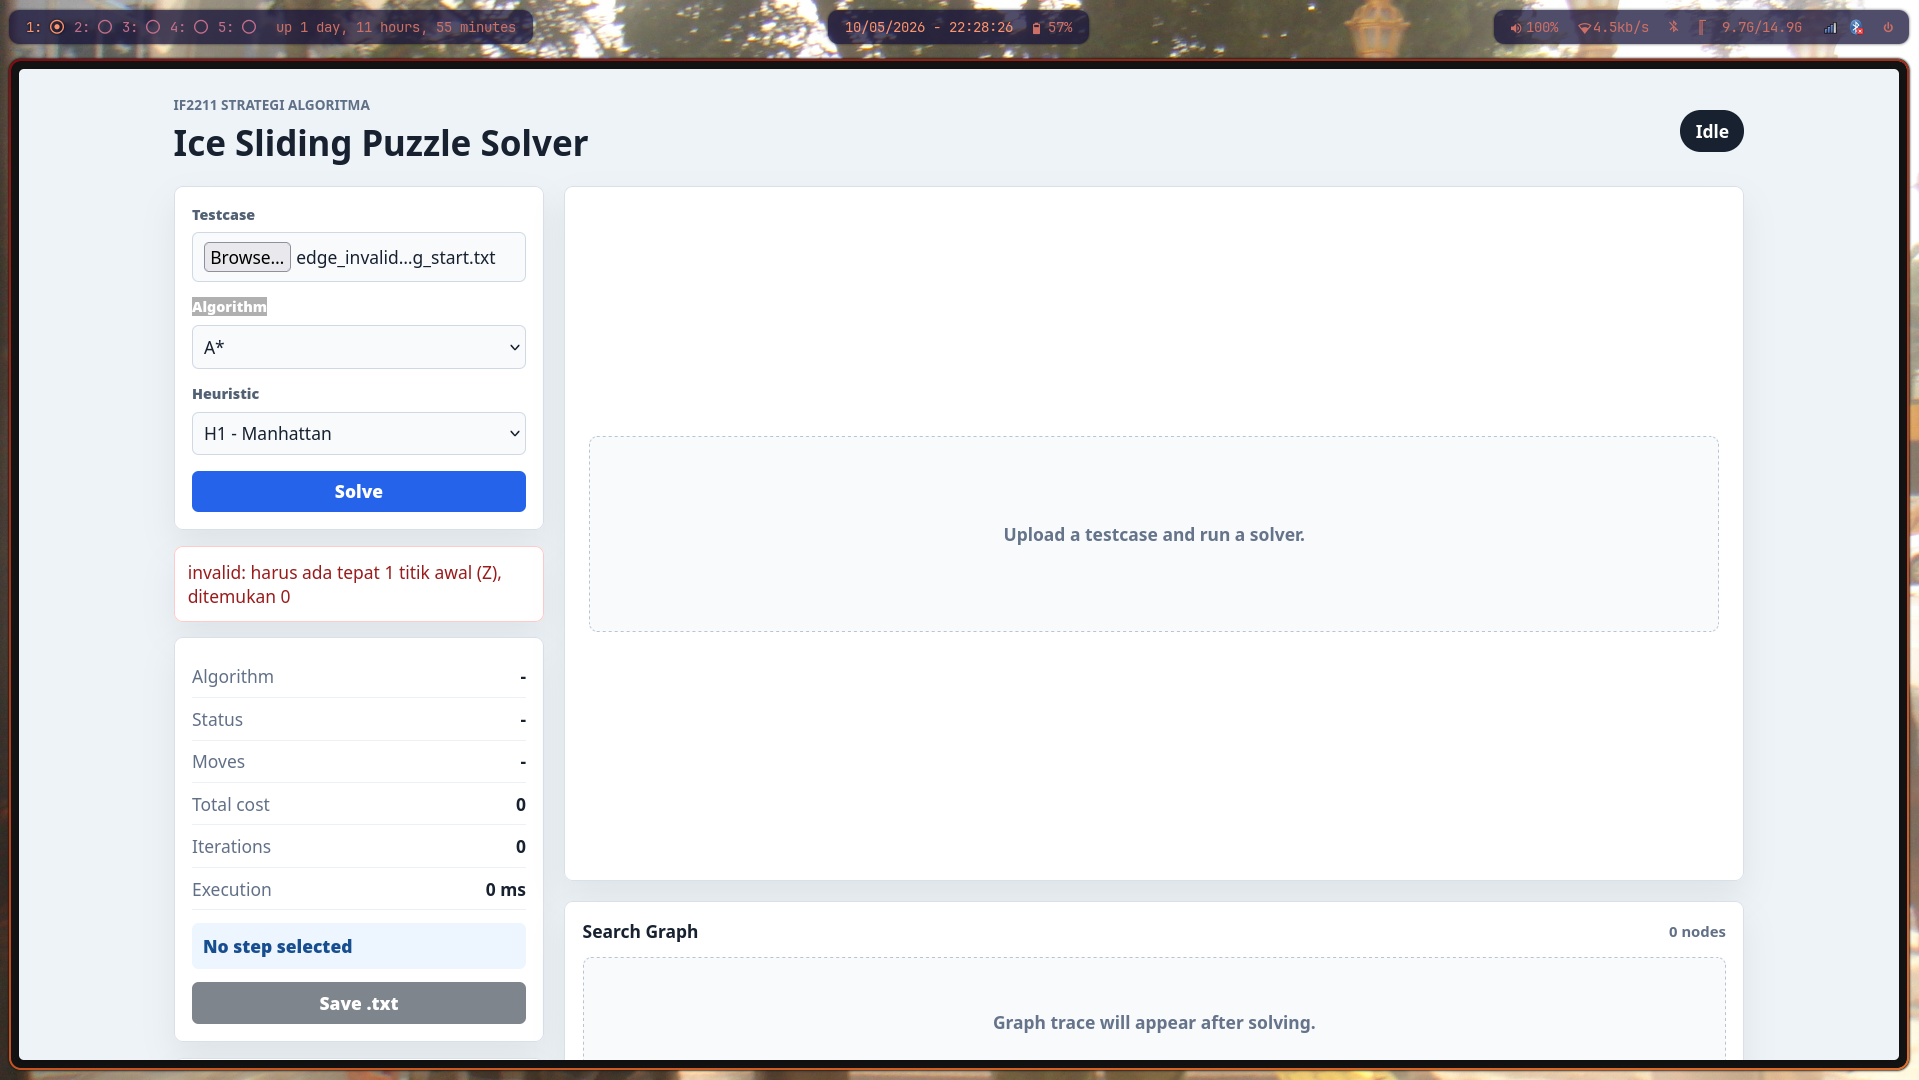
\includegraphics[width=0.85\textwidth]{figures/testcase_invalid_start.png}
    \caption{Bukti GUI error handling untuk input tanpa start}
\end{figure}

\begin{figure}[H]
    \centering
    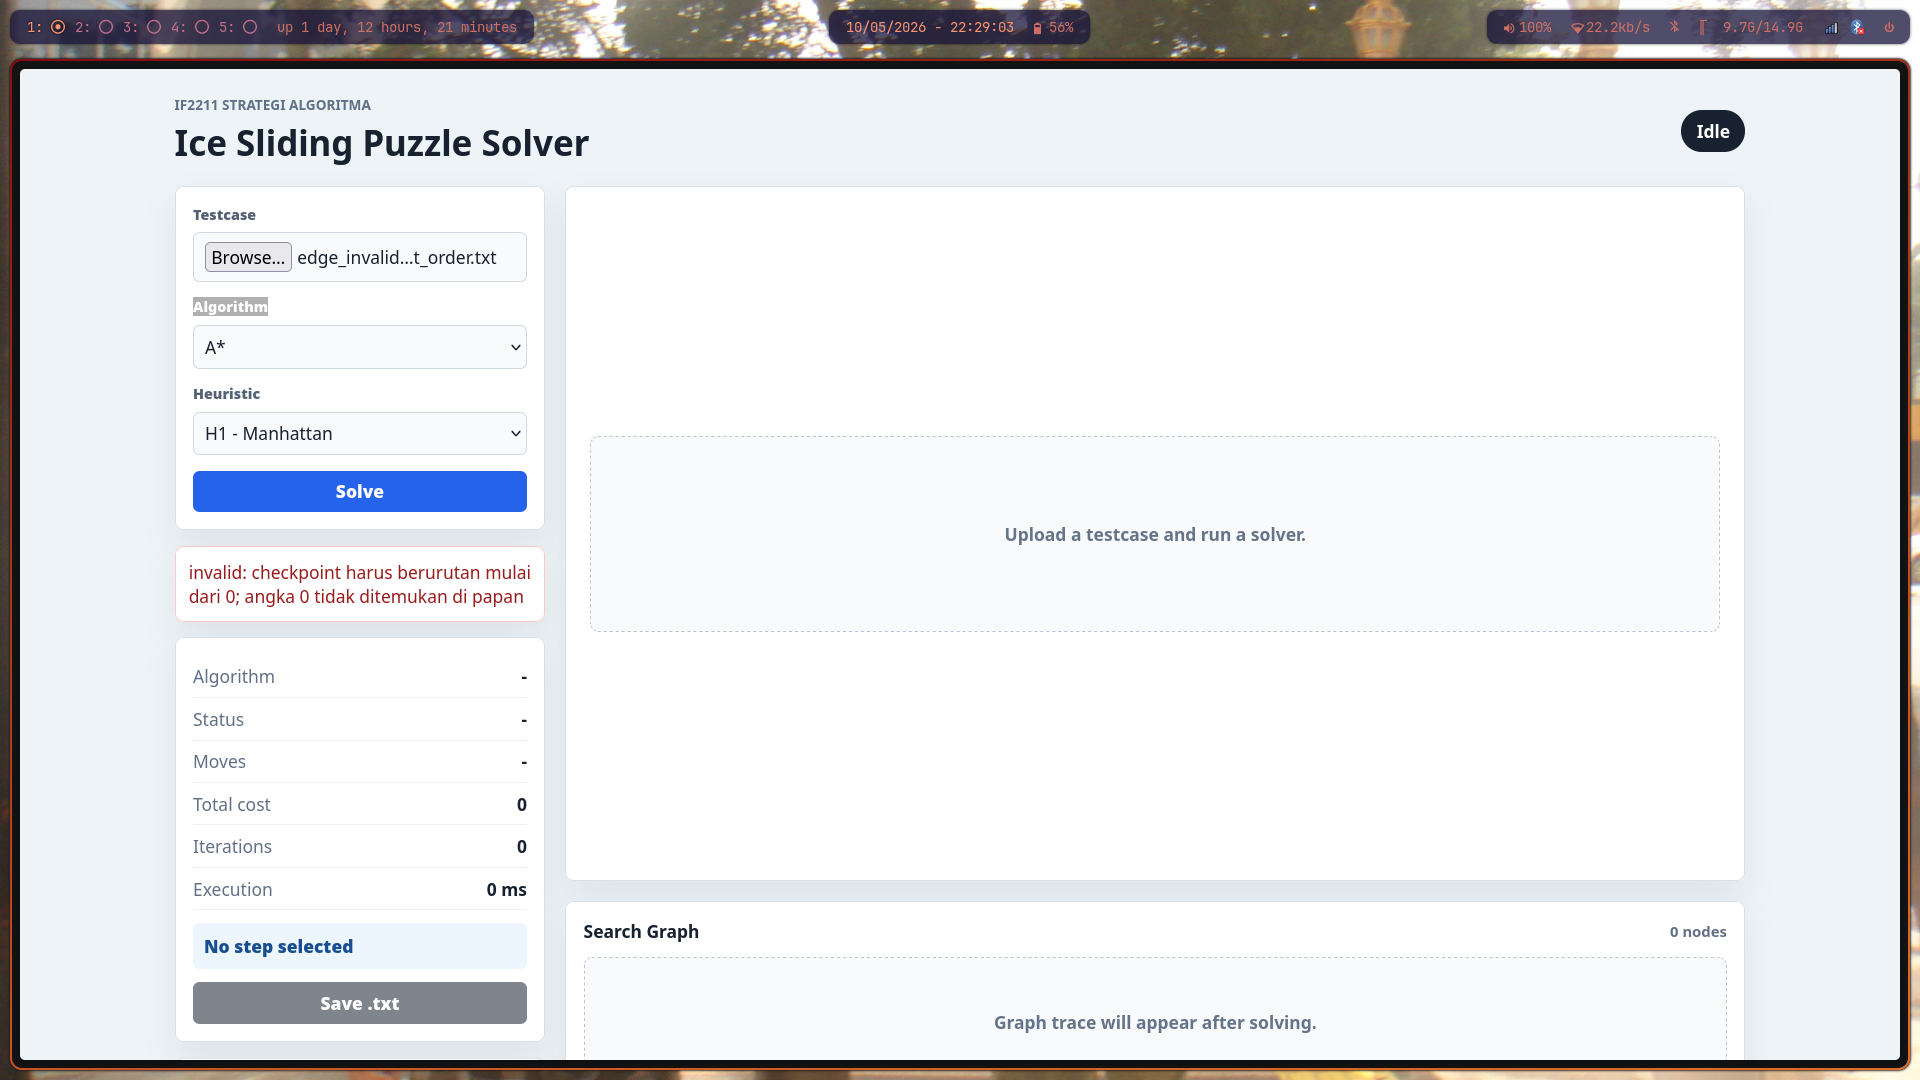
\includegraphics[width=0.85\textwidth]{figures/testcase_invalid_order.png}
    \caption{Bukti GUI error handling untuk urutan checkpoint tidak valid}
\end{figure}

\begin{figure}[H]
    \centering
    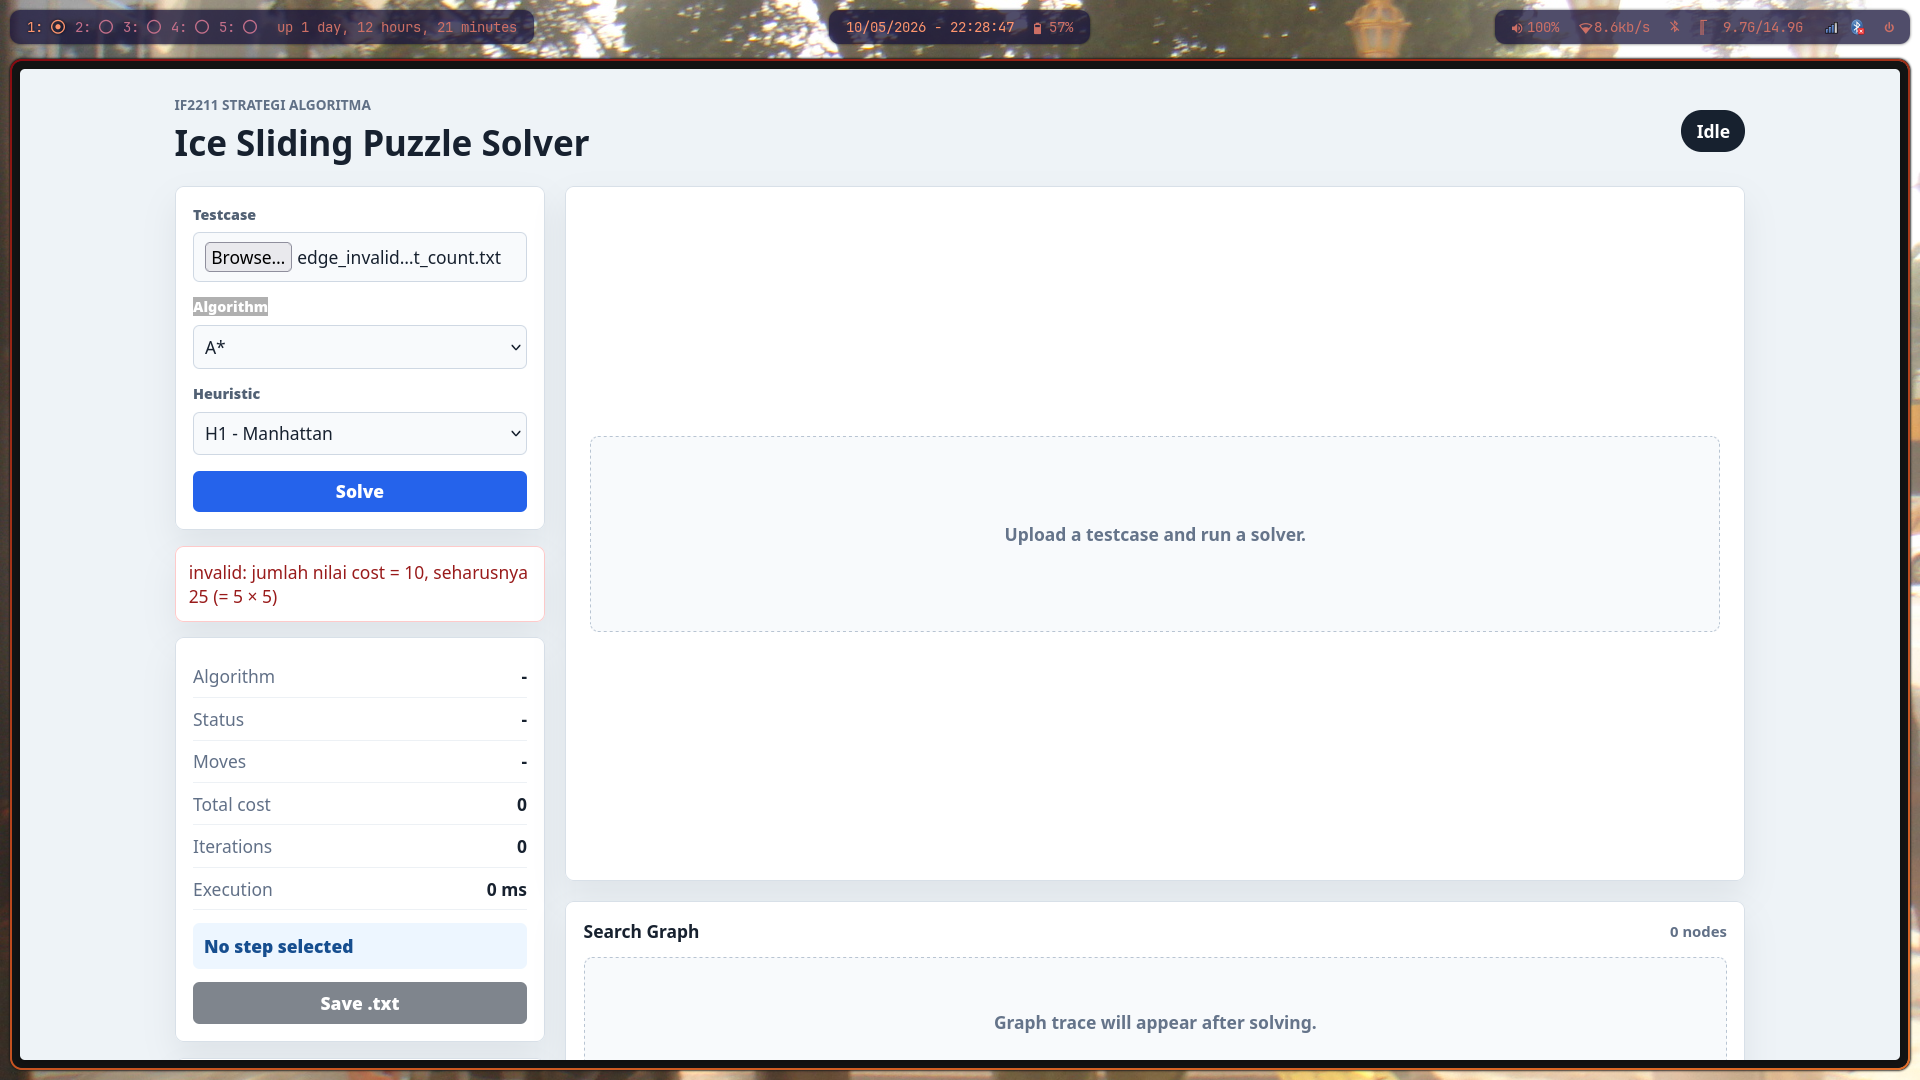
\includegraphics[width=0.85\textwidth]{figures/testcase_invalid_cost.png}
    \caption{Bukti GUI error handling untuk jumlah cost tidak valid}
\end{figure}

\subsection{Ringkasan Hasil Pengujian}\label{sub:Hasil Pengujian}

\begin{table}[H]
    \centering
    \begin{tabular}{|c|L{4cm}|c|c|c|c|}
        \hline
        \textbf{No} & \textbf{Kasus} & \textbf{Algoritma} &
        \textbf{Heuristic} & \textbf{Status GUI} & \textbf{Bukti} \\
        \hline
        1 & UCS testcase & UCS & - & Lulus & Gambar UCS \\
        \hline
        2 & GBFS testcase & GBFS & H1, H2, H3 & Lulus & Gambar GBFS H1--H3 \\
        \hline
        3 & A* testcase & A* & H1, H2, H3 & Lulus & Gambar A* H1--H3 \\
        \hline
        4 & DFS testcase & DFS & - & Lulus & Gambar DFS \\
        \hline
        5 & BFS testcase & BFS & - & Lulus & Gambar BFS \\
        \hline
        6 & Edge case dan error handling & - & - & Lulus & Gambar error handling \\
        \hline
    \end{tabular}
    \caption{Ringkasan hasil pengujian GUI}
\end{table}
